%%% -*-LaTeX-*-

\chapter{Mathematical Rolling Model}

Because transient interactions with agonist-coated blood vessel
surfaces and the resulting cell rolling is critical in the early
activation of a platelet, we want a model that describes both the
physics of fluid and bond forces and the chemistry of bond formation
and breaking during this process. Rolling velocity is often measured
and interpreted as a proxy for cell contact with a surface during
rolling because it is relatively easy to observe, whereas directly
experimentally measuring the number of bonds between a platelet and
surface is not feasible. 

\section{Problem Description}
\label{sec:problem-description}

Below I describe the set of assumptions that we use to model a
platelet translocating along an agonist-coated surface. Important,
experimentally variable, biological and physical parameters such as
receptor and ligand density, receptor on/off rates, shear rate, and
fluid viscosity appear in the model.

\begin{figure}
  \centering
  \begin{tikzpicture}[scale=2]
  \newcommand{\dist}{0.5}
  \newcommand{\Length}{2.5}
  \newcommand{\slope}{0.5}
  \newcommand{\buff}{0.1}

  % Define a coordinate for the center of the platelet, and draw a
  % node there
  \coordinate (pltcenter) at (0, 1 + \dist);
  \node [circle, inner sep=1.5pt, fill=black] at (pltcenter) {};

  % Draws the wall and the platelet
  \draw (-\Length, 0) -- (\Length, 0);
  \draw (pltcenter) circle [radius = 1];
  \draw[<->] (0, .05) -- node[right] {$\separation$} (0, \dist-.05);
  \draw[<->] (-.15, .05) -- node[left] {$\height$} (-.15,
  .95+\dist);
  \draw[dashed] (0, 1+\dist) -- (-.3, 1+\dist);

  % Draws the lines showing the applied velocities
  \draw[->] (pltcenter) ++(1+\buff, 0) -- node[above] {$\velocity$}
  (\Length-\buff, 1+\dist);

  \draw[->] (0, 1+\dist) ++(135:1+\buff) arc [start angle=135, end
  angle=45, radius=1+\buff] node[midway, above] {$\rotation$};

  % Draws the arrows showing the shear flow
  \foreach \y in {0.5, 1, 1.5, 2, 2.5}
     \draw[->] (-\Length, \y) -- (-\Length + \slope*\y, \y);
  
  \draw[gray, very thin] (-\Length, 0) -- node[near start, right,
  black] {$\tn{Shear rate} = \shear$} (-\Length + \slope*\Length,
  \Length);

  % Draws a bond between the platelet and wall
  \draw[decorate, decoration=zigzag] (pltcenter) ++(315:1)
  node[circle, inner sep=1.5pt, fill=black] {} -- (1.25,0) node
  [circle, inner sep=1.5pt, fill=black] {};

  % Labels the x and theta coordinates
  \draw[{Bar[]}->] (0, -\buff) -- node[fill=white] {$\wallDist$}
  (1.25, -\buff);

  \draw (pltcenter) -- +(0, -1);
  \draw (pltcenter) -- node[above right] {$R$} +(315:1);
  \draw[->] (pltcenter) ++(0, -3*\buff) arc [start angle=270, end
  angle=315, radius=3*\buff] node[midway, below] {$\recAngle$};
\end{tikzpicture}

  \caption{Model geometry}
  \label{fig:model-geometry}
\end{figure}

\subsection{Geometry and Physics}
\label{sec:geometry-physics}

A sketch of the problem geometry is given in Figure
\ref{fig:model-geometry}. Assume we have a circular rigid platelet (of
radius $\radius$) rolling and translating in shear flow with shear
rate $\shear$ adjacent to a wall. The platelet translates parallel to
the wall at speed $\velocity$, and rolls at angular velocity
$\rotation$. Because the circle is always translating parallel to the
wall, there is a fixed vertical distance $\separation$ between the
wall and the closest point on the circle. Define the height $\height$
of the platelet to be the distance from the wall to the center of the
platelet ($\height = \separation + \radius$). The fluid forces exerted
on the platelet are a function of $\height$, $\radius$, $\shear$, and
$\velocity$, as well as the fluid viscosity ($\viscosity$) which is
constant across all experiments. We assume that the platelet is moving
in a Stokes flow, meaning that the inertial terms are negligible and
force balance must be satisfied on the platelet at all times.

Due to the linearity of Stokes equations, there is a linear
relationship between platelet velocity and fluid force. In a general
3D Stokes flow, this relationship is given by a $6 \times 6$ matrix
equation $\mathbf{F} = \underline{\underline{R}} \mathbf{U}$ where
$\mathbf{U}$ is a $6 \times 1$ vector containing the 3 translational
velocities and 3 rotational velocities, and $\mathbf{F}$ is a
$6 \times 1$ vector containing the 3 forces and 3 torques. However in
the current model we've made a number of simplifying assumptions.
\begin{enumerate}
\item The flow is a 2D Stokes flow, eliminating all forces and
  translational velocities along the dimension going into and out of
  the page. This also eliminates rotations and torques about the two
  other dimensions. Similarly the platelet geometry is a circle in
  2D. We arrive at this assumption by assuming the platelet is a
  sphere in 3D, but due to the length-dependence of bond formation and
  breaking there is only a narrow reactive strip of width $\width$
  along the bottom of the platelet in which bonds exist. We then
  approximate this narrow reaction region with a finite cylinder of
  height $\width$ and radius $\radius$. 
\item The platelet remains at a constant separation distance from the
  wall, eliminating all vertical motion (and consequently we ignore
  all vertical forces imposed by bonds between the platelet and
  wall). In published adhesive dynamics models, the nonspecific
  repulsive forces between the platelet and vessel wall are only
  significant at very short ranges, therefore it is plausible to say
  that at the length scales relevant to the problem, the height of the
  platelet from the surface does not change, and bond forces pulling
  the platelet towards the wall are balanced by the nonspecific
  repulsive forces.
\item The hydrodynamic forces on the platelet are computed assuming
  the platelet is infinitely far from the wall. In particular the
  translational velocity of the platelet is assumed to be independent
  of the torque, and vice versa. This assumption is hard to justify
  physically, and there is a good case for removing this assumption
  from the model in the future, however it does simplify the
  relationship between bond forces and torques and the platelet
  translation and angular velocities. 
\end{enumerate}
With these assumptions in place, we end up with two decoupled linear
equations relating the horizontal force ($\horzTotalForce$) to the
translational velocity ($\velocity$) and relating the torque
($\totalTorque$) to the rotational velocity ($\rotation$):
\begin{align}
  \label{eq:force-bal}
  0 &= \velFriction(\appliedVel - \velocity) + \horzTotalForce \\
  \label{eq:torque-bal}
  0 &= \rotFriction(\appliedRot - \rotation) + \totalTorque
\end{align}
% Equations.
% NOTE: I will need to expand on this more when I add equations to
% the paper. I also forgot to discuss the applied fluid velocities.

We identify bonds by their two attachment points on the wall and on
the platelet surface, so each bond has two coordinates associated with
it for each of its endpoints. Points on the wall are given by the
coordinate $\wallDist$, defined to be the horizontal distance from the
center of the circle, and points on the platelet surface are given by
the coordinate $\recAngle$, defined to be the angle formed by the
receptor, the center of the circle, and the closest point on the
circle to the wall (Figure \ref{fig:model-geometry}). With this
definition of $\wallDist$ and $\recAngle$, the distance from a ligand at
$\wallDist$ on wall and a receptor $\recAngle$ on the platelet surface is
given by the equation
\begin{equation}
  \label{eq:dim-length}
  \length^2 (\wallDist, \recAngle) \equiv (\radius - \radius\cos\recAngle +
  \separation)^2 + (\radius\sin\recAngle - \wallDist)^2.
\end{equation}

\subsection{Biology}
\label{sec:biology}

The platelet surface is covered with receptors at an angular density
of $\receptorDensity$ receptors/radian, and bonds can form between
points on the surface of the circle and points on the wall. The number
of ligand binding sites on the substrate is assumed to be in
excess. We assume that bonds act like Hookean springs with a rest
length of 0, so the force exerted by a bond is proportional to its
length and the proportionality constant is the stiffness of the
bond. Formation and dissociation rates are distance and force
dependent, respectively. We use the Bell model \cite{Bell1978} to
express the bond dissociation rate as a function of force, and the
Dembo model \cite{Dembo1988} to express the bond formation rate as a
function of the distance between a receptor and ligand. This gives us
the following equations for formation rate and dissociation rate:
\begin{align}
  \label{eq:binding}
  \onRate(\length) &= \onConst \exp
                     \left(-\frac{\stiffness}{2\boltzmann\temp}
                     \length^2(\wallDist, \recAngle) \right), \\
  \label{eq:unbinding}
  \offRate(\length) &= \offConst \exp \left( \frac{\stiffness
                      \length(\wallDist, \recAngle)}{\refForce} \right).
\end{align}

In order to calculate $\horzForce$ and $\torque$ for an existing set
of bonds between the platelet and wall, we simply have to add up the
individual contributions to the force and torque from each bond. The
force and torque generated by an individual bond can be derived from
the geometry of the model along with the assumption that the force
vector $\mathbf{F}$ points in the same direction as the bond with
magnitude proportional to the bond length. I'll leave out the
derivation. The horizontal force generated by a single bond
($\horzForce$) is given simply by
\begin{equation}
  \label{eq:horz-force}
  \horzForce = \stiffness (\wallDist - \radius\sin\recAngle),
\end{equation}
while the torque generated by a single bond ($\torque$) is given by
the slightly more complicated
\begin{equation}
  \label{eq:torque}
  \torque = -\stiffness \radius ((\radius - \radius\cos\recAngle +
  \separation)\sin\recAngle + (\radius\sin\recAngle - \wallDist)\cos\recAngle).
\end{equation}

\section{Deterministic PDE model}
\label{sec:determ-pde-model}

If we assume that there is a continuous distribution of bonds between
the platelet and the wall, we can define the function
$\bondDensity(\wallDist, \recAngle, \dTime)$ which gives the density of
bonds at time $\dTime$ between points $\wallDist$ and $\recAngle$ on the
wall and platelet, respectively. Bonds advect in $\wallDist$ with
velocity $\velocity$ and they advect in $\recAngle$ with velocity
$\rotation$. Bonds form at the rate given in equation
(\ref{eq:binding}) and saturate in $\recAngle$ with a maximum density
$\receptorDensity$. Finally, bonds break at the force-dependent rate
given in equation (\ref{eq:unbinding}). Putting all of this together
gives us the following PDE definition of $\bondDensity$:
\begin{equation}
  \label{eq:bond-density}
  \Pder{\bondDensity}{\dTime} = \rotation
  \Pder{\bondDensity}{\recAngle} + \velocity
  \Pder{\bondDensity}{\wallDist} + \onRate(\length)
  \left(\receptorDensity - \DimReceptorSaturation \right) -
  \offRate(\length) \bondDensity(\wallDist, \recAngle, \dTime).
\end{equation}

This equation can't yet be solved for $\bondDensity$, because there
are still 2 unknowns in it: $\velocity$ and $\rotation$. Recall from
above that $\velocity$ and $\rotation$ are found by balancing the
fluid and bond forces acting on the platelet (equations
(\ref{eq:force-balance}) and (\ref{eq:torque-balance})). First, we
have to calculate the total force $\horzTotalForce$ and torque
$\totalTorque$ generated by the distribution of bonds $\bondDensity$:
\begin{align}
  \label{eq:horz-total-force}
  \horzTotalForce &= \DimQuantity{\horzForce}, \\ 
  \label{eq:total-torque}
  \totalTorque &= \DimQuantity{\torque}
\end{align}

Once we have $\horzTotalForce$ and $\totalTorque$, the platelet velocities
$\velocity$ and $\rotation$ are given by the equations:
\begin{align}
  \label{eq:force-balance}
  0 &= \velFriction (\appliedVel - \velocity) + \horzTotalForce, \\
  \label{eq:torque-balance}
  0 &= \rotFriction (\appliedRot - \rotation) + \totalTorque.
\end{align}

Now we have 3 equations in 3 unknowns and this is a closed system that
can be solved simultaneously for $\bondDensity$, $\velocity$, and
$\rotation$. We still need to define the domains of all three
variables, and give boundary conditions for $\bondDensity$ before we
can solve this system. Assume that bonds can only attach to the lower
half-circle of the platelet surface, while bonds can form at any point
along the wall. Thus we are solving $\bondDensity$ in the domain
$(-\infty, \infty) \times [-\pi/2, \pi/2]$. We need to enforce
boundary conditions at the upstream (with respect to variables
$\wallDist$ and $\recAngle$) ends of the $\wallDist$ and $\recAngle$
domains. Because we assume there are no bonds attached to the upper
half of the platelet, and because the equilibrium concentration of
bonds $\bondDensity \rightarrow 0$ as $L \rightarrow \infty$, we must
set homogeneous Dirichlet boundary conditions on both $\wallDist$ and
$\recAngle$. Finally we just set the initial condition to be
$\bondDensity(\wallDist, \recAngle, 0) \equiv \bondDensity_0(\wallDist,
\recAngle)$.

In order to eliminate some parameters, we nondimensionalize this model
by introducing nondimensional coordinates
$\wallDist = \radius \ndWallDist$ and $\ndTime = \offConst \dTime$
(note that $\recAngle$ is already dimensionless) and nondimensional
functions $\radius \bondDensity = \receptorDensity \ndBondDensity$,
$\velocity = \radius \offConst \ndVelocity$, and
$\rotation = \offConst \ndRotation$. The details of the
nondimensionalization are included in Appendix \ref{app:nondim}, but
the final nondimensional set of equations is
\begin{align}
  \nonumber
  \Pder{\ndBondDensity}{\ndTime}
  &= \ndRotation \Pder{\ndBondDensity} {\recAngle} + \ndVelocity
    \Pder{\ndBondDensity}{\ndWallDist} + \ndOnConst \exp
    \left(-\frac{\onForceScale}{2} \ndLength^2(\ndWallDist, \recAngle)
    \right) \left(1 - \NDReceptorSaturation\right) \\
  \label{eq:nd-bond-density}
  &\qquad - \exp
    \left(\offForceScale\ndLength(\ndWallDist, \recAngle)\right)
    \ndBondDensity(\ndWallDist, \recAngle, \ndTime), \\
  \label{eq:nd-force-balance}
  0 &= \ndVelFriction \left(\ndAppliedVel - \ndVelocity\right) + 
      \ndHorzTotalForce, \\
  \label{eq:nd-torque-balance}
  0 &= \ndRotFriction \left(\ndAppliedRot - \ndRotation\right) +
      \ndTotalTorque.
\end{align}

The nondimensional bond length $\ndLength$ is given by
\begin{equation}
  \label{eq:nd-length}
  \ndLength^2(\ndWallDist, \recAngle) = (1 - \cos\recAngle +
  \ndSeparation)^2 + (\sin\recAngle - \ndWallDist)^2,
\end{equation}
and the nondimensional force $\ndHorzTotalForce$ and torque
$\ndTotalTorque$ are given by
\begin{align}
  \label{eq:nd-force}
  \ndHorzTotalForce &= \NDQuantity{(\ndWallDist - \sin\recAngle)} \\
  \label{eq:nd-torque}
  \ndTotalTorque &= \NDQuantity{\left[ \left(1 - \cos\recAngle +
                   \ndSeparation\right) \sin\recAngle +
                   \left(\sin\recAngle - \ndWallDist\right)
                   \cos\recAngle \right]}
\end{align}
A complete list of the nondimensional coordinates, functions, and
parameters with their definitions are given in Table
\ref{tab:nd-vars}.

\section{Stochastic model}
\label{sec:stochastic-model}

An assumption that is implicit in the deterministic model is that cell
rolling is mediated by a large number of bonds between the platelet
and the surface, and therefore by the law of large numbers randomness
of bond formation and breaking is inconsequential. This assumption is
not supported by previous rolling models, nor is it supported by
experimental observation. In \cite{Wang2013}, which models platelet
rolling along vWF, at no point during their numerical experiment does
the number of bonds between the platelet and surface exceed 9. Even in
models of leukocyte rolling, where the drag force on the cell is
several times greater than drag on a platelet, the number of bonds
between the cell and the surface is approximately 20 at any given
point in time.

Therefore, there is good evidence that rolling is mediated by a small
number of bonds that can halt a platelet, and the implicit assumption
in the deterministic model that there are many bonds is not valid. In
order to fully and accurately describe platelet rolling, we must model
bond formation and breaking as a stochastic process, and consequently
the rolling velocity of the platelet is a stochastic process.

For the stochastic model---like the deterministic model---assume that
there are $\receptorDensity$ receptors per radian, and the receptors
are uniformly distributed along the surface of the platelet. Assume
there is an excess of ligand on the wall surface, so that bonds can
form anywhere along the wall and there is no saturation of bonds in
the $\wallDist$ dimension.

A bond can form between a receptor located at $\recAngle$ and a point
$\wallDist$ on the wall at ``rate'' $\onRate(\wallDist,
\recAngle)$. More precisely, the time $t_\tn{form}$ that it takes a
bond to form between $\wallDist$ and $\recAngle$ is exponentially
distributed with mean $1/\onRate(\wallDist, \recAngle)$. Similarly,
the time it takes a bond between $\recAngle$ and $\wallDist$ to break
is exponentially distributed with mean
$1/\offRate(\wallDist, \recAngle)$. Finally, a single bond between
$\wallDist$ and $\recAngle$ generates horizontal force and torque
which are given by $f_h$ and $\tau_s$ as defined in equations
(\ref{eq:horz-force}) and (\ref{eq:torque}). As in the continuous
model, assume that only bonds on the lower half-circle of the platelet
can interact with the wall surface.

One way to simulate this model would be to track each of the
$2\pi \receptorDensity$ receptors on the surface of the platelet,
whether they are bound or unbound. But this is expensive to do, so I
do something else. At the beginning of a simulation, I partition the
entire platelet surface $\theta \in [-\pi, \pi)$ into $2N$
subintervals of equal length
$I_j(0) = \left[-\frac{\pi} + \frac{\pi}{N}j, -\frac{\pi} +
  \frac{\pi}{N} (j+1)\right)$. Each subinterval has width
$\nu \equiv \pi/N$. Within each subinterval $I_j$, there are
$b_\tn{max} \equiv \receptorDensity \pi/N$ total receptors, which are
all assumed to be located at the midpoint $\binMidpoint{j}$ of the
interval:
$\binMidpoint{j}(0) \equiv -\frac{\pi}{2} + \frac{\pi}{N} \left( j +
  \frac{1}{2} \right)$. As the simulation evolves, the intervals $I_j$
(and their midpoints $\binMidpoint{j}$) track with the surface of the
platelet as it rotates; that is, they form a Lagrangian partition of
the platelet surface (see Figure \ref{fig:plt-bins}).

\begin{figure}
  \centering
  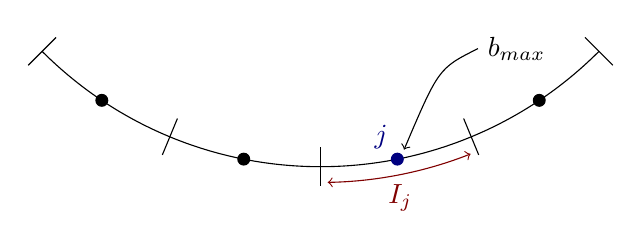
\begin{tikzpicture}
  [scale=5,
  midpoints/.style=blue!50!black,
  intervals/.style=red!50!black]
  \draw (225:1) arc [start angle=225, end angle=315, radius=1];
  \foreach \th in {-2,...,2}
  \draw (270 + 22.5*\th:.95) -- (270 + 22.5*\th:1.05);

  \foreach \th in {236.25,258.75,303.75}
  \filldraw (\th:1) circle [radius=.015];
  
  \filldraw[midpoints] (281.25:1) node [above left] {$\binMidpoint{j}$}
  circle [radius=.015];

  \draw [<->, intervals] (271:1.04) arc [start angle=271, end
  angle=291.5, radius=1.04] node [midway, below] {$I_j$};

  \draw[->] (.4,-.7) node [right,fill=white] {$b_\tn{max}$}
  .. controls (.3, -.75) .. (282.5:.98);
\end{tikzpicture}

  \caption{Partition of (part of) the platelet surface}
  \label{fig:plt-bins}
\end{figure}

To simulate random bond breaking, a random number is generated for
each existing bond to test if it breaks within the time step
$\Delta \dTime$. The probability that a bond between $\wallDist$ and
$\binMidpoint{j}$ in the time interval $[\dTime, \dTime + \Delta \dTime)$
is $\mathbb{P} = 1 - \exp(-\Delta \dTime \offRate(\wallDist,
\binMidpoint{j}))$.

Next look at bond formation. The probability of a bond forming between
points $\binMidpoint{j}$ and $\wallDist$ can be split into two distinct
probabilities: the probability that a bond forms from a receptor at
position $\binMidpoint{j}$ to anywhere on the wall (denote this event as
$A$, and the associated probability as $\mathbb{P}(A)$), and the
probability that a bond forms to the point $\wallDist$ on the wall
from any receptor (denote this event as $B$, and the probability
$\mathbb{P}(B)$). The probability of the combined event $A \cap B$ is
\begin{equation}
  \label{eq:joint-prob}
  \mathbb{P}(A \cap B) = \Delta t (b_\tn{max} - n_j)
  \onRate(\wallDist, \binMidpoint{j}).
\end{equation}


% To simulate bond formation, first assume that at most 1 bond can
% form in a single time step in each subinterval $I_j$. One can think of
% bond formation 

% Then for each
% subinterval, calculate the probality of a bond forming within that
% subinterval in the time interval $\Delta \dTime$. If a bond forms then an
% $\wallDist$ is chosen at random.

First, the probability that a bond forms within subinterval $I_j$ is
given by the rate of bond formation multiplied by the number of
available receptors in $I_j$. The rate that bonds form from
$\binMidpoint{j}$ to \emph{any} point on the wall, integrate $\onRate$
with respect to $\wallDist$. In the case $\onRate(\wallDist,
\binMidpoint{j}) = k_\tn{on} \exp\left(-\frac{\stiffness
    \length^2}{2\boltzmann \temp}\right)$, we have
\begin{equation}
  \label{eq:total_fm_rate}
  \int_{-\infty}^{\infty} \onRate(\wallDist, \binMidpoint{j})\, dx = k_\tn{on} \exp
  \left( -\frac{\stiffness}{2\boltzmann \temp} (\radius - \radius
    \cos\binMidpoint{j} + \separation)^2 \right) \sqrt{\frac{2 \pi
      \boltzmann \temp}{\stiffness}}.
\end{equation}
Therefore the probability that a bond forms somewhere in the interval
$I_j$ to any point on the wall in a time interval of length $\Delta t$
is given by 
\begin{equation}
  \label{eq:form-prob}
  \mathbb{P}(A) = \Delta t (b_\tn{max} - \bondDensity_j) \left[ \onConst
    \exp \left( - \frac{\stiffness}{2 \boltzmann \temp} \left( \radius
        - \radius\cos\binMidpoint{j} + \separation \right)^2 \right)
    \sqrt{\frac{2\pi \boltzmann \temp}{\stiffness}} \right].
\end{equation}

Next, we need to find the probability that a bond forms between a
point $\wallDist$ on the wall and $\binMidpoint{j}$, given that a bond forms from
$\binMidpoint{j}$. From the definition of conditional probability,
\begin{align}
  \mathbb{P} \left( B \mid A \right) 
  &= \frac{\mathbb{P}(A \cap B)}
  {\mathbb{P}(A)} \nonumber \\
  \label{eq:wall-distr}
  &= \sqrt{\frac{\stiffness}{2\pi \boltzmann\temp}} \exp
    \left(-\frac{\stiffness}{2 \boltzmann \temp} \left(\wallDist -
    \radius \sin{\binMidpoint{j}} \right) \right).
\end{align}
That is if a bond is forming from a receptor at the point
$\binMidpoint{j}$ on platelet, the probability distribution of its wall
attachment point $\wallDist$ is a normal distribution with mean
$\sin\binMidpoint{j}$ and variance $\boltzmann\temp/\stiffness$:
$\wallDist \sim \mathcal{N} \left(\mu=\sin\binMidpoint{j},
  \sigma^2 = \boltzmann\temp/\stiffness \right)$.

Just like the deterministic algorithm, the stochastic algorithm tracks
3 time-varying unknowns: bonds between the platelet and wall,
translational velocity, and angular velocity. However now the bonds
between the platelet and surface are tracked discretely, and the bond
quantity between points $x$ and $\theta$ is now a stochastic
process. Both velocities are also stochastic processes as well,
because of their dependence on the bonds between the platelet and
wall.

A full description of the stochastic algorithm is given in Appendix
\ref{cha:numerical-schemes}, but I will summarize the key features
below.
\begin{enumerate}
\item Platelet-wall bonds are tracked in an array which stores the two
  endpoints of each bond. Each row represents a single bond; the first
  column stores the $x$ coordinate of the bond (the wall attachment
  point), and the second column stores $j$ (the $\theta$-bin from which
  the bond formed.
  \begin{equation}
    \label{eq:bond-list}
    \verb|bond_list| =
    \begin{bmatrix}
      x_0(t) & j_0 \\
      x_1(t) & j_1 \\
      \vdots & \vdots \\
      x_{\texttt{nbonds}-1}(t) & j_{\texttt{nbonds} - 1}
    \end{bmatrix}    
  \end{equation}
  where $j_i = 0, \hdots, 2N-1$ and $\Der{x_i}{t} = -V(t)$ for $i = 0,
  \hdots, \texttt{nbonds} - 1$.

  As time evolves, \verb|bond_list| is updated in two ways: (1) the
  $x$-coordinate changes as the platelet moves, and (2) rows are added
  to or removed from \verb|bond_list| as bonds form or break.

\item For each time step, we carry out the following steps:
  \begin{enumerate}
  \item Update $x_i(t)$ and $\binMidpoint{j}(t)$.
  \item Compute the rate of bond formation $\onRate(\binMidpoint{j})
    b_j^\tn{avail}$ for $j = 0, \hdots, 2N-1$ and the rate of bond
    breaking $\offRate(x_i, \binMidpoint{j_i})$ for $i = 0, \hdots,
    \texttt{nbonds} - 1$.
  \end{enumerate}
\end{enumerate}
